\documentclass{beamer}

\usetheme{Baba}

\usetikzlibrary{overlay-beamer-styles}

\hypersetup{
  colorlinks=true,
  urlcolor=blue,
  linkcolor=babadarkblue,
  citecolor=blue
}
\renewcommand{\UrlFont}{\normalfont}


\title{Supporting the treatment of Alzheimer's patients with explainable artificial intelligence}
\date{\today}
\author{Esten H. Leonardsen}

\begin{document}
    \begin{frame}
        \titlepage
    \end{frame}

    \begin{frame}{Background}
        \begin{tikzpicture}
            \node[] at (-5.25, 3.5) {};
            \node[] at (5.25, -3.5) {};

            \only<1>{
                \node[inner sep=0pt, draw=black] at (0, 0) {
                    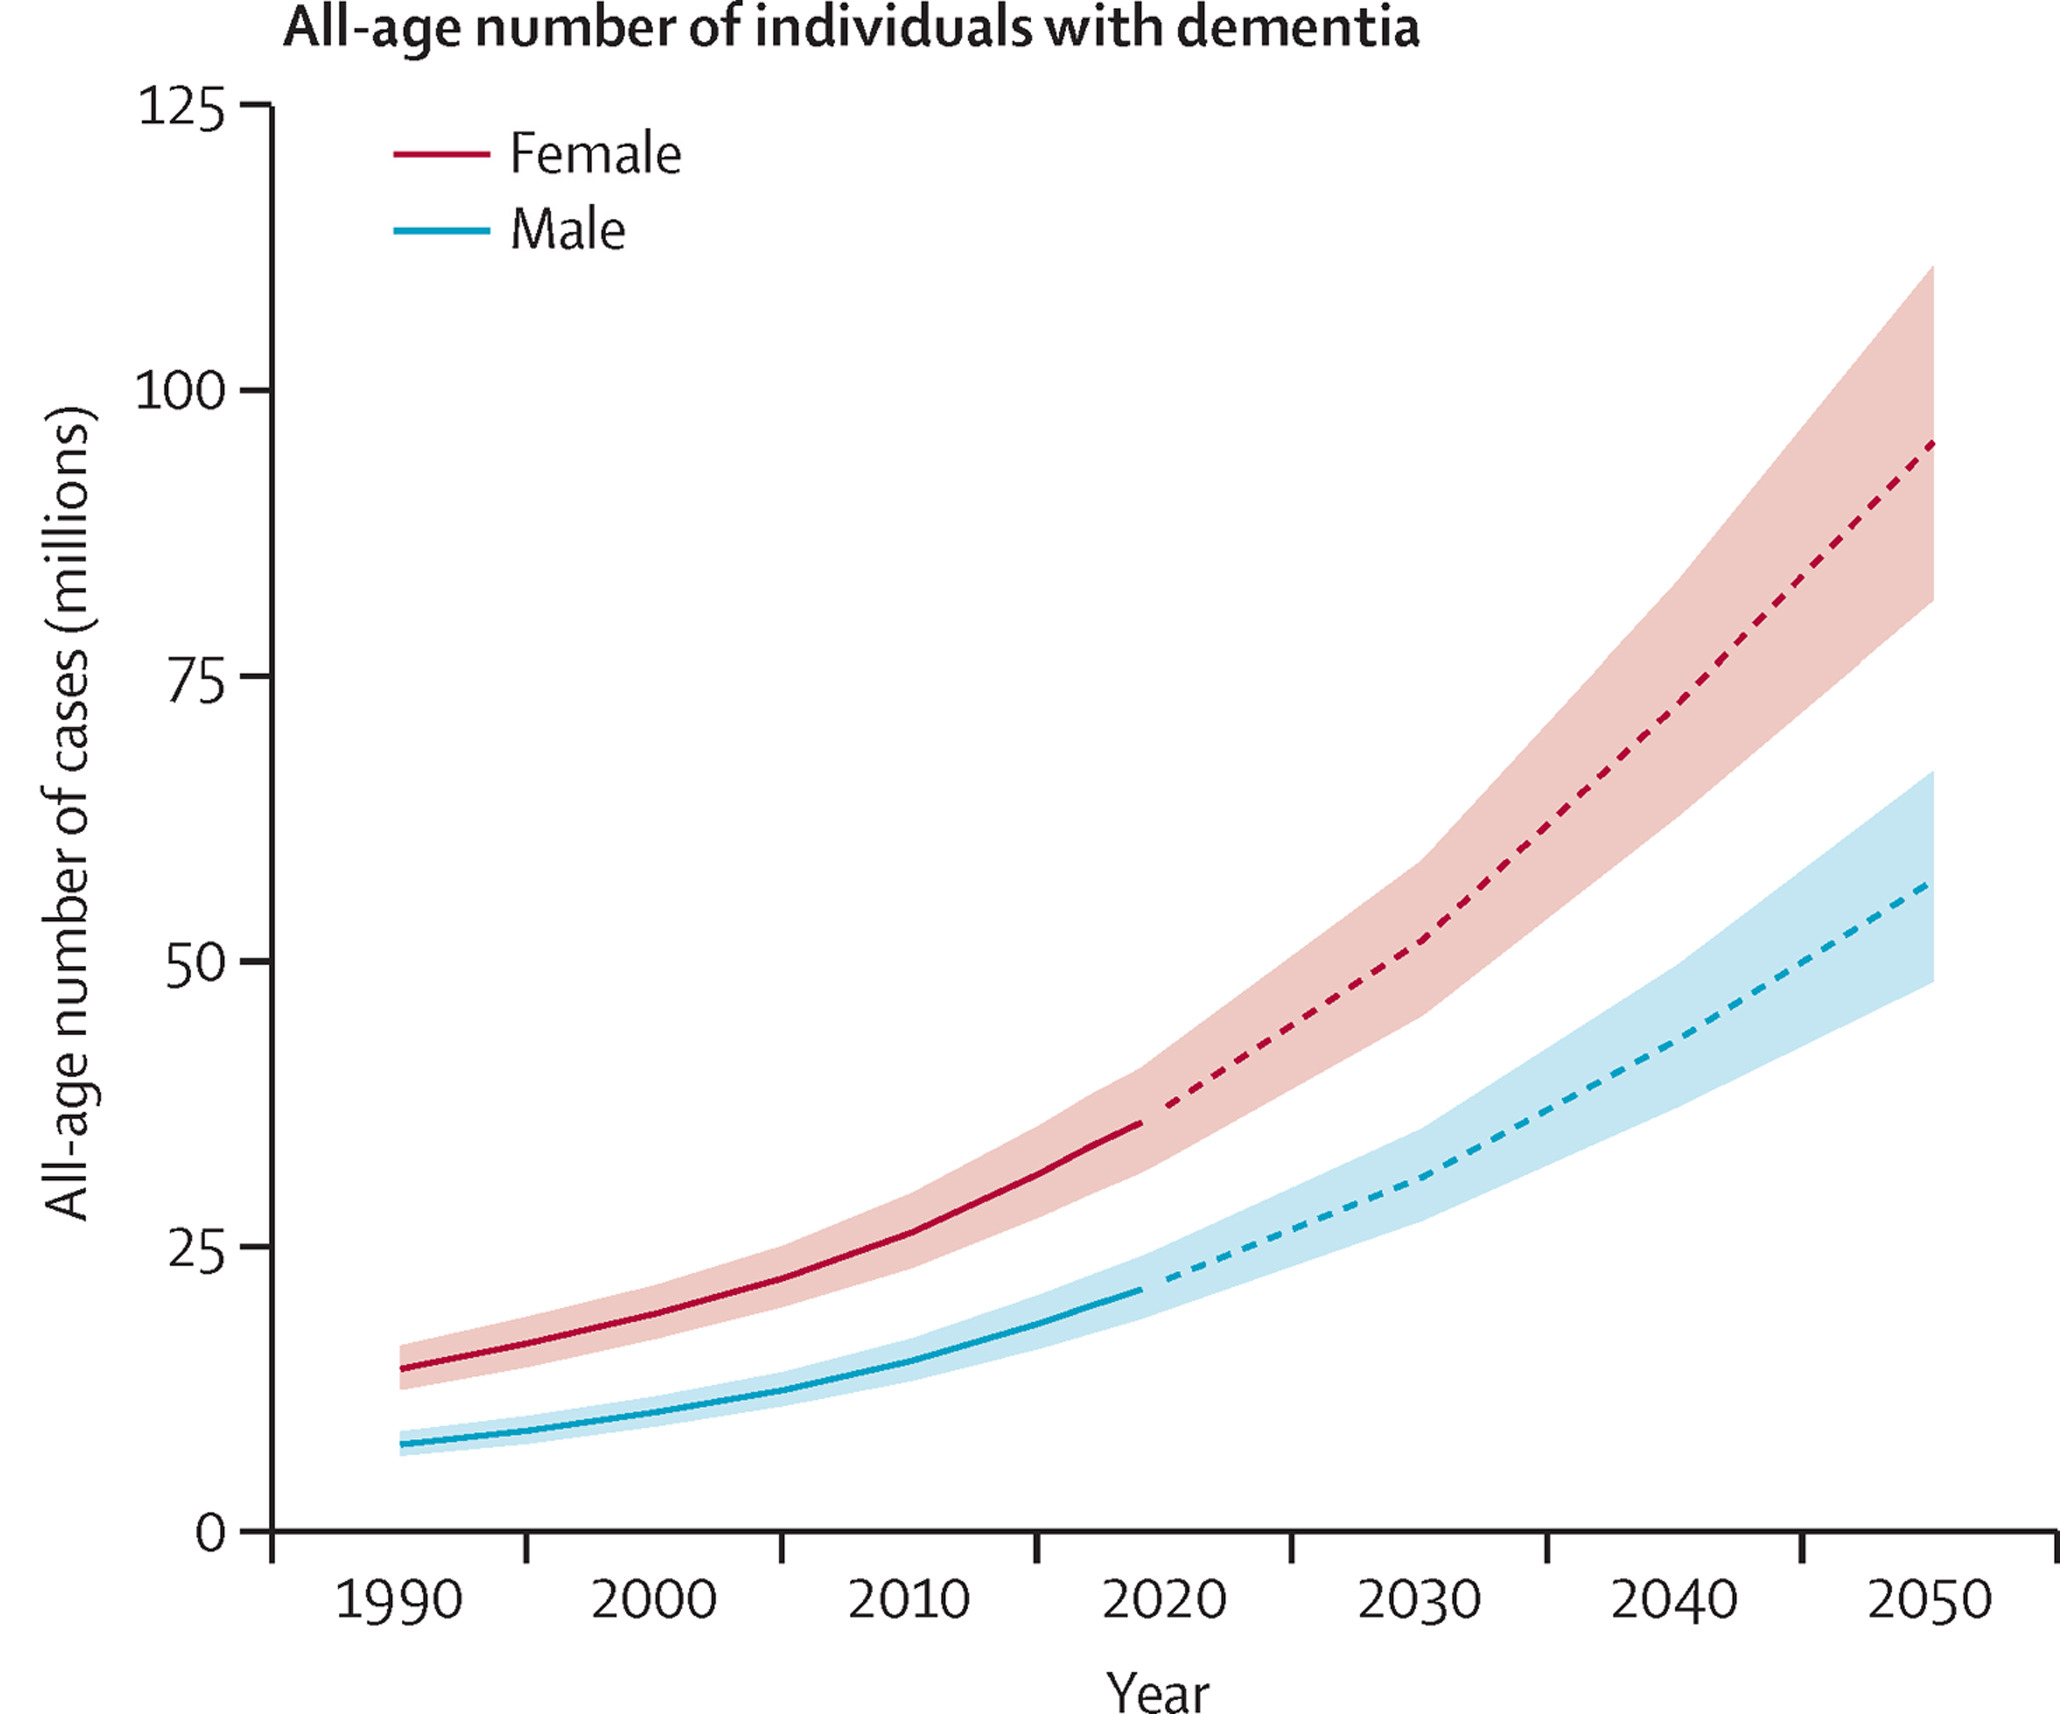
\includegraphics[width=6cm]{data/prevalence.jpg}
                };
                \node[anchor=south, font=\tiny, text width=10cm, align=flush center] at (0, -3.75) {
                    Global Burden of Disease Dementia Forecasting Collaborators (2022). Estimation of the global prevalence of dementia in 2019 and forecasted prevalence in 2050: an analysis for the Global Burden of Disease Study 2019. \textit{The Lancet Public Health}.
                };
            }
            \only<2>{
                \node[inner sep=0pt, draw=black] at (0, 0) {
                    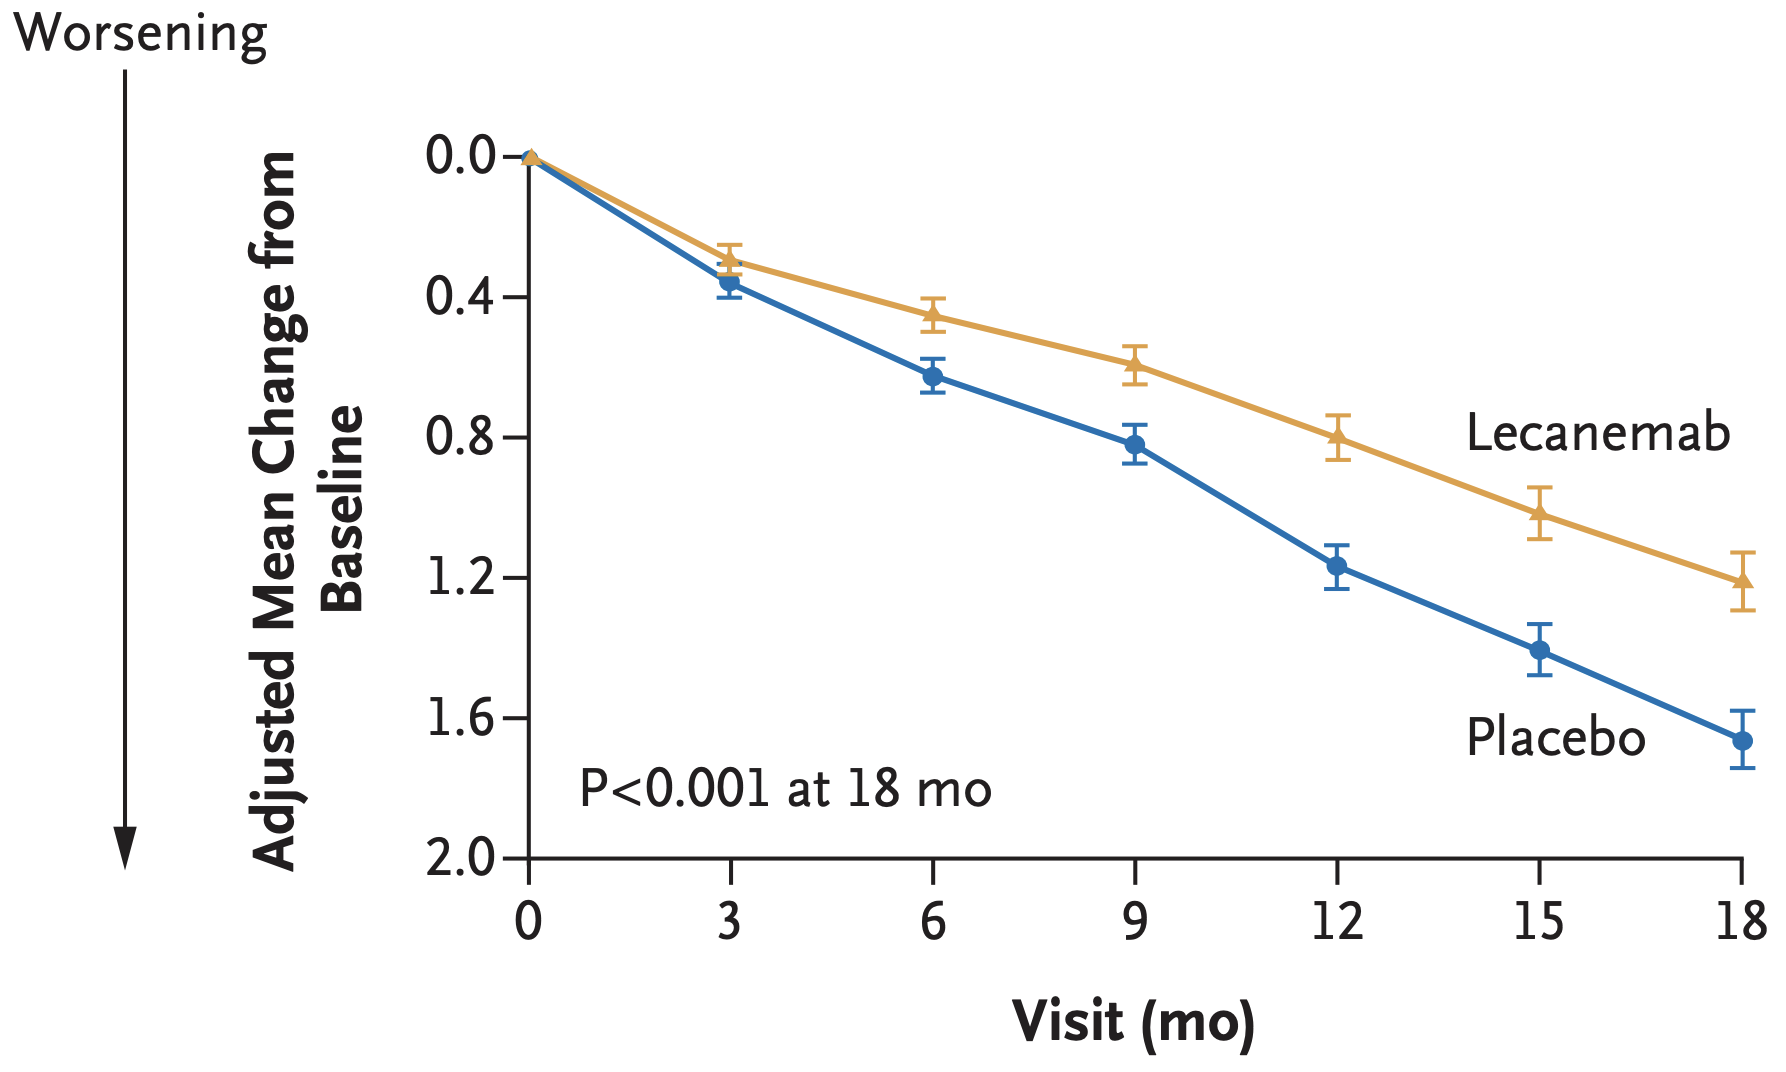
\includegraphics[width=8.5cm]{data/worsening.png}
                };
                \node[anchor=south, font=\tiny, text width=10cm, align=flush center] at (0, -3.75) {
                    Van Dyck, C. H., Swanson, C. J., Aisen, P., Bateman, R. J., Chen, C., Gee, M., ... \& Iwatsubo, T. (2023). Lecanemab in early Alzheimer’s disease. \textit{New England Journal of Medicine}.
                };
            }
            \only<3>{
                \node[inner sep=0pt, draw=black] at (0, 0) {
                    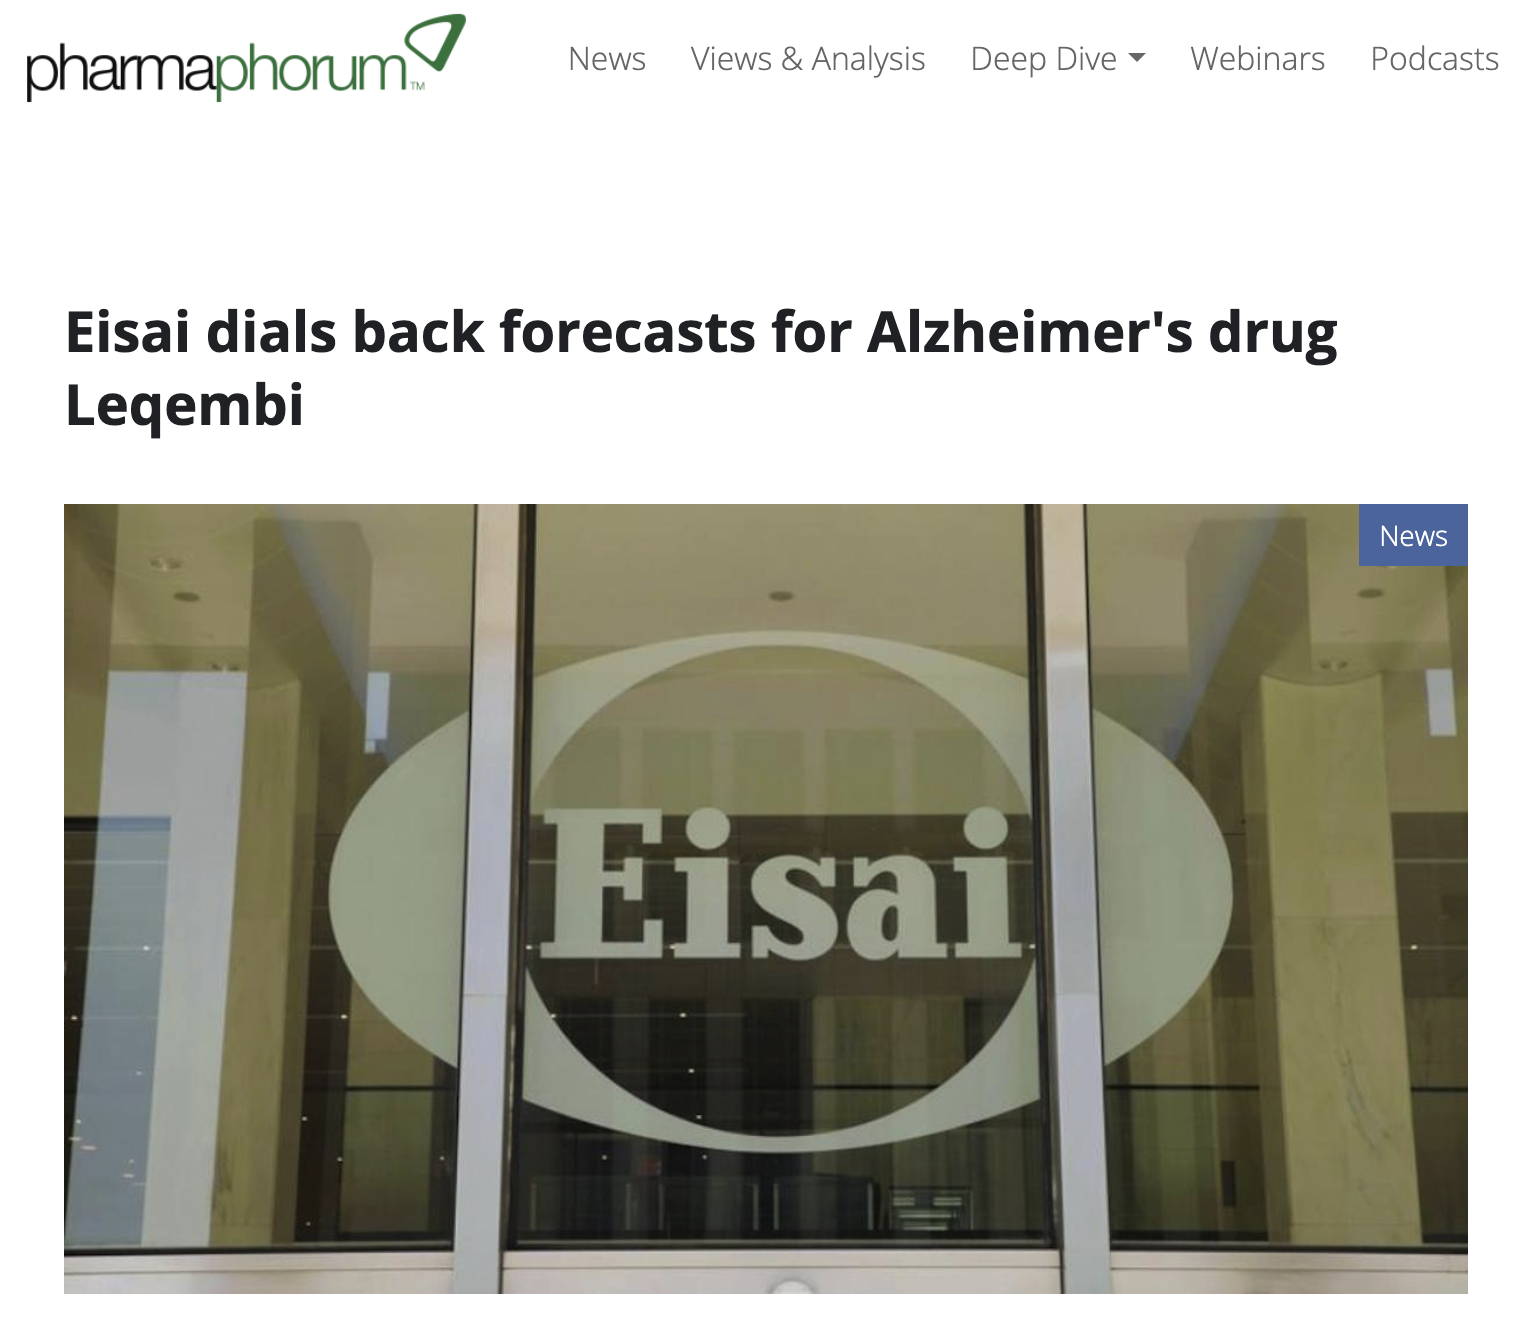
\includegraphics[width=7cm]{data/eisai.png}
                };
            }
            \only<4>{
                \node[] at (0, 0) {
                    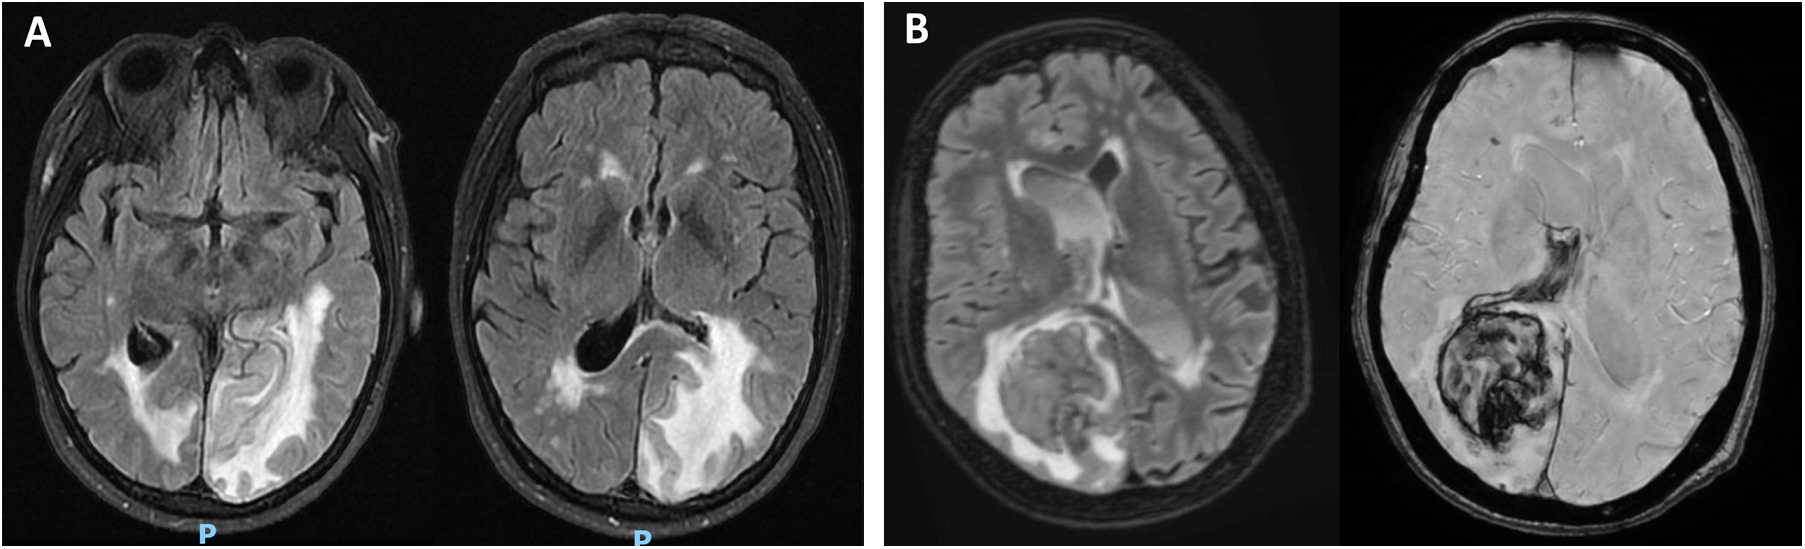
\includegraphics[width=10cm]{data/aria.jpg}
                };
                \node[anchor=south, font=\tiny, text width=10cm, align=flush center] at (0, -3.75) {
                    Villain, N., Planche, V., \& Levy, R. (2022). High-clearance anti-amyloid immunotherapies in Alzheimer's disease. Part 1: Meta-analysis and review of efficacy and safety data, and medico-economical aspects. \textit{Revue neurologique}.
                };
            }
        \end{tikzpicture}
    \end{frame}

\end{document}
